\documentclass{article}
\usepackage[italian]{babel}
\usepackage[T1]{fontenc}
\usepackage{graphicx}
\usepackage[utf8x]{inputenc}
\usepackage{amsmath}
\usepackage{amsthm}
\usepackage{hyperref}
\date{27 Novembre 2018}
\author{Lorenzo Cavuoti}
\title{Oscillatore sinusoidale a ponte di Wien con OpAmp}

\begin{document}
	\maketitle
	
	\paragraph{0)}
	Lo scopo dell'esperienza è realizzare un oscillatore sinusoidale a ponte di Wien. Ho montato il primo circuito di figura \ref{fig:circuiti}, i componenti, misurati con il multimetro digitale, risultano:
	\begin{itemize}
		\item $R1=9.89\pm0.08k\Omega$
		\item $R2=9.91\pm0.08k\Omega$
		\item $R3=10.05\pm0.08k\Omega$
		\item $R4=9.81\pm0.08k\Omega$
		\item $R5=9.81\pm0.08k\Omega$
		\item $Rpot=10.63\pm0.08k\Omega$
		\item $C1=10.2\pm0.4nF$
		\item $C2=10.2\pm0.4nF$
	\end{itemize}

	\begin{figure}
		\centering
		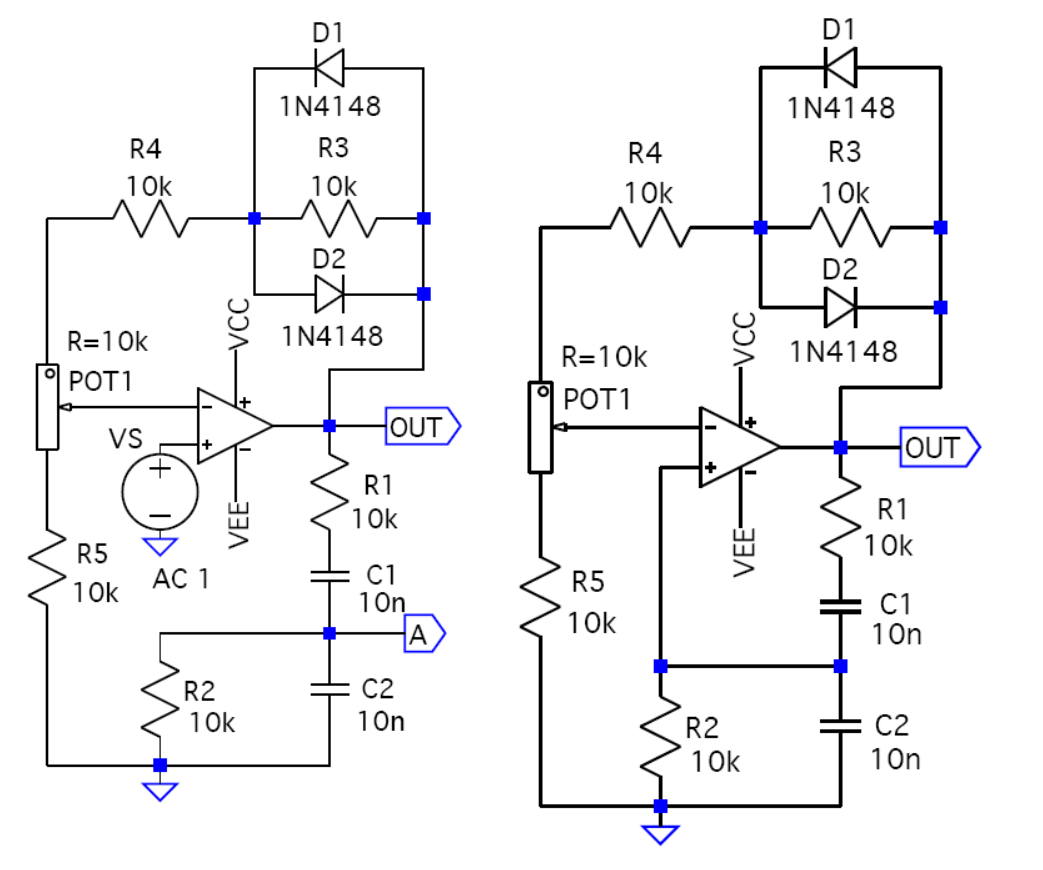
\includegraphics[width=0.9\linewidth]{figure/circuiti}
		\caption{Schema circuitale dei due circuiti usati nell'esperienza, a destra l'oscillatore a ponte di Wien}
		\label{fig:circuiti}
	\end{figure}

	\paragraph{1)}
	Ho alimentato l'OpAmp con $V_{CC}=14.88\pm0.08V$ e $V_{EE}=-15.09\pm0.08V$ e ho inviato all'ingresso un segnale sinusoidale di ampiezza $V_S=260\pm10 mV$, successivamente ho variato la frequenza tra circa 0.5kHz e 3kHz e per ciascun valore ho misurato l'ampiezza e lo sfasamento di $V_A$, i dati presi sono riportati in tabella \ref{tab:guadagno} e \ref{tab:fase} e nel grafico \ref{fig:grafico}.
	Lo sfasamento risulta nullo per $f_{0mis}=1.61\pm0.06$ kHz, l'errore è stato stimato variando la frequenza fino a quando non si notava uno sfasamento tra $V_S$ e $V_A$, il valore è in accordo con la teoria $f_{0att}=1/2\pi R_1 C_1 = 1.57\pm0.06$kHz. Successivamente si è tenuta la frequenza costante e si è girato il potenziometro, si nota che quando la resistenza verso terra del potenziometro aumenta il guadagno diminuisce, e viceversa, come previsto dalla teoria. Infine mantenendo la frequenza del segnale di ingresso a $f_0$ e aumentando $V_{Spp}=4.1\pm0.2V$ si ha $V_{App} = 3.4\pm0.1V$ (pp indica l'ampiezza picco picco), il guadagno per $f=f_0$ quindi diminuisce all'aumentare dell'ampiezza.
	
	
	\begin{table}
	\centering
	\begin{tabular}{cccc}
		\hline
		f[kHz]&$V_{Spp}$ [mV]&$V_{App}$ [mV]&$\beta A_V$\\
		\hline
		$0.52\pm0.005$ & $510\pm20$ & $370\pm20$ & $0.73\pm0.04$ \\
		$0.723\pm0.007$ & $510\pm20$ & $440\pm20$ & $0.86\pm0.06$ \\
		$0.946\pm0.009$ & $510\pm20$ & $480\pm20$ & $0.94\pm0.06$ \\
		$1.40\pm0.01$ & $510\pm20$ & $510\pm20$ & $1.00\pm0.06$ \\
		$1.93\pm0.02$ & $510\pm20$ & $510\pm20$ & $1.00\pm0.06$ \\
		$2.34\pm0.02$ & $510\pm20$ & $500\pm20$ & $0.97\pm0.06$ \\
		$2.90\pm0.03$ & $510\pm20$ & $480\pm20$ & $0.93\pm0.06$ \\
	\end{tabular}
	\caption{Tabella dell'open loop gain $\beta A_V$ in funzione della frequenza di $V_{in}$}
	\label{tab:guadagno}
	\end{table}

	\begin{table}
		\centering
		\begin{tabular}{cc}
			\hline
			f[kHz]&fase [gradi] \\
			\hline
			$0.511\pm0.005$ & $45.7\pm0.5$ \\
			$0.706\pm0.007$ & $34.6\pm0.4$ \\
			$0.964\pm0.01$ & $22.5\pm0.3$ \\
			$1.44\pm0.01$ & $7.66\pm0.09$ \\
			$2.14\pm0.02$ & $-7.63\pm0.08$ \\
			$2.90\pm0.03$ & $-19.2\pm0.2$ \\
		\end{tabular}
	\caption{Tabella della fase in funzione della frequenza di $V_{in}=510\pm20mV$}
	\label{tab:fase}
	\end{table}

\begin{figure}
	\centering
	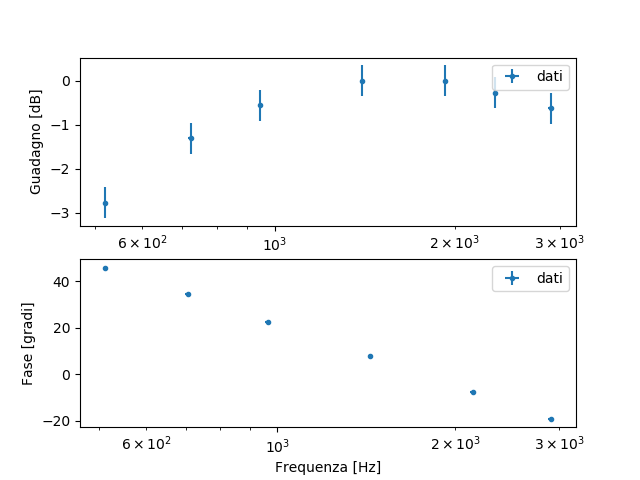
\includegraphics[width=1\linewidth]{figure/grafico.png}
	\caption{Grafico dell'open loop gain e della fase in funzione della frequenza}
	\label{fig:grafico}
\end{figure}

\paragraph{2)}
Ho collegato il terminale positivo di ingresso dell'OpAmp alla rete di feedback disconnettendo il generatore (secondo ciruito di figura \ref{fig:circuiti}). Il segnale $V_{out}$ presenta una forma sinusoidale (figura \ref{fig:2sinusoide}), inoltre si nota che girando il potenziometro in senso orario, quindi aumentando la resistenza verso terra, l'ampiezza di $V_{out}$ diminuisce, fino ad avere un segnale piatto. Invece se si gira il potenziometro il senso antiorario, ovvero diminuendo la resistenza verso terra, l'ampiezza di $V_{out}$ aumenta, se si gira ancora la sinusoide viene leggermente distorta, fino ad avere clipping a $V_{outpp}=28\pm1 V$ figura \ref{fig:2clipping}

\begin{figure}
	\centering
	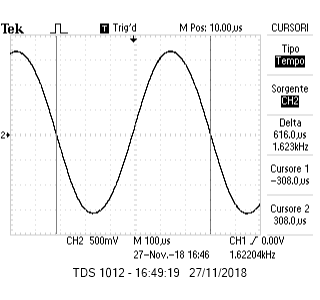
\includegraphics[width=0.6\linewidth]{figure/2sinusoide}
	\caption{Segnale sinusoidale di $V{out}$}
	\label{fig:2sinusoide}
\end{figure}

\begin{figure}
	\centering
	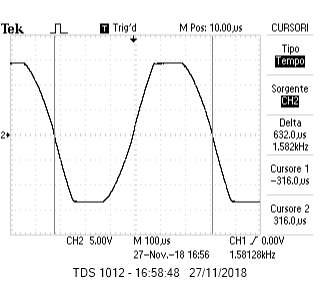
\includegraphics[width=0.6\linewidth]{figure/2clipping}
	\caption{Clipping di $V_{out}$}
	\label{fig:2clipping}
\end{figure}

\paragraph{3)}
La frequenza di oscillazione risulta $f=1.62\pm0.01$kHz, ottenuta invertendo la misura del periodo con i cursori, la frequenza è in accordo con la teoria con la misura del punto 1. Si nota inoltre che la frequenza non dipende dalla tensione di alimentazione dell'OpAmp e neanche dalla posizione del potenziometro finchè non si ha clipping: se il segnale presenta clipping la frequenza aumenta, come si nota in figura \ref{fig:2clipping}. Variando la posizione del potenziometro il valore del segnale che cambia maggiormente risulta l'ampiezza di $V_{out}$.

\paragraph{4)}
Ho posizionato il potenziometro in modo da creare il segnale $V_{out}$ con minore ampiezza possibile, successivamente ho staccato la rete di feedback e connesso il generatore di funzioni con un segnale sinusoidale di ampiezza $V_{inpp}=0.51\pm0.02$V misurata con l'oscilloscopio, il segnale in uscita risulta $V_{outpp}=1.53\pm0.06$V $A_V=3.0\pm0.2$ compatibile con il guadagno atteso dalla teoria $A_V=3$ per ottenere $\beta A_V=1$

\paragraph{5)}
E'stato ricollegato il circuito del punto 2 togliendo però i diodi, si osserva che $V_{out}$ passa da un segnale piatto alla saturazione variando la posizione del potenziometro, senza la possibilità di avere un segnale di ampiezza intermedia, in particolare se $|V_{CC}|>|V_{EE}|$ si ha saturazione in basso (figura \ref{fig:5satbasso}), invece se $|V_{CC}|<|V_{EE}|$ si ha saturazione in alto (figura \ref{fig:5satalto}), tuttavia più $|V_{CC}|-|V_{EE}|$ è piccolo meno clipping si ha, fino a non essere più visibile con l'oscilloscopio. Si nota anche che la frequenza di oscillazione rimane la stessa entro l'incertezza di misura del tempo dell'oscilloscopio.\newline
 I due diodi svolgono il ruolo di limitare l'ampiezza del segnale in uscita, infatti quando $V_{out}>V_{th}$ (dove con $V_{th}$ si indica la tensione di soglia del diodo) il diodo ha una resistenza molto minore di $R_3$ e possiamo considerare la caduta di potenziale trascurabile ai capi del resistore. Successivamente questo segnale rientra nell'OpAmp che amplifica la differenza tra V- e V+ ma a causa del diodo l'ampiezza di V- è variata poco rispetto a V+, di conseguenza l'ampiezza del segnale in uscita diminuisce.


\begin{figure}
	\centering
	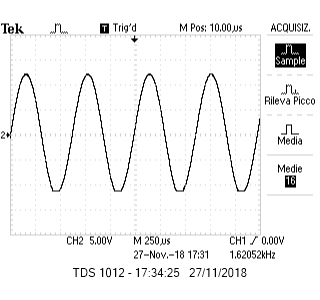
\includegraphics[width=0.6\linewidth]{figure/5satBasso}
	\caption{Saturazione in basso di $V_{out}$ per $|V_{CC}|>|V_{EE}|$}
	\label{fig:5satbasso}
\end{figure}

\begin{figure}
	\centering
	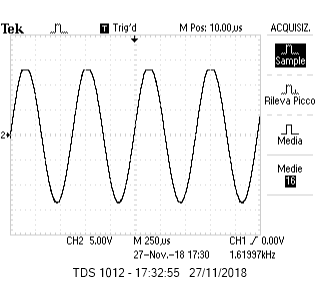
\includegraphics[width=0.6\linewidth]{figure/5satAlto}
	\caption{Saturazione in alto di $V_{out}$ per $|V_{CC}|<|V_{EE}|$}
	\label{fig:5satalto}
\end{figure}

\end{document}

